\documentclass{beamer}
\usetheme{Madrid}
\renewcommand{\raggedright}{\leftskip=0pt \rightskip=0pt plus 0cm}

\usepackage{tikz}
\usetikzlibrary{positioning, shapes.geometric, arrows.meta}
\usepackage{multicol}
\usepackage{graphicx}
\usepackage{xcolor}
\usepackage{array}
\usepackage{amsmath}
\usepackage{booktabs}

\title{Comparative Study of Segmentation-Guided Self-Supervised Learning
for Chest X-ray Representation}
\author[Aysha Rishana K, M4 SPE]{}
\date[\today]{}

\begin{document}

%-----------------------------------
% TITLE SLIDE
%-----------------------------------
\begin{frame}
\titlepage{}
\vspace{-2.5cm}
\begin{center}
    \textbf{Final Presentation of M.Tech Main Project}
\end{center}
\vspace{0.3cm}
\begin{columns}[T,totalwidth=\textwidth]
\hspace{.4cm}
  \column{0.33\textwidth}
  Guided by\\
  \textbf{Prof.Nishil Kumar P.P.}\\
  Dept. of ECE\\
  GCE Kannur

  \column{0.33\textwidth}
  \centering
  \includegraphics[scale=0.5]{college logo.jpeg}

  \column{0.33\textwidth}
  Presented by\\
  \textbf{Aysha Rishana K}\\
  M.Tech : SPE \\
  Semester: S4\\
  Roll No: 4
\end{columns}
\begin{center}
\textbf{Department of Electronics and Communication Engineering\\Government College of Engineering Kannur}
\end{center}
\end{frame}

%-----------------------------------
% CONTENTS
%-----------------------------------
\begin{frame}
\frametitle{Contents}
\tableofcontents
\end{frame}


%===================================================================
\section{Introduction}
%===================================================================

\begin{frame}{Introduction}
\begin{itemize}
    \item Chest X-rays are the most commonly performed diagnostic imaging examination worldwide.
    \vspace{4pt}
    \item Automated disease detection requires large \textbf{expert-annotated} datasets, which are expensive and scarce.
    \vspace{4pt}
    \item \textbf{Self-Supervised Learning (SSL)} enables AI models to learn useful features from \textbf{unlabeled} images.
    \vspace{4pt}
    \item Standard SSL methods treat all image regions equally --- but diseases mainly appear in the \textbf{lung fields}.
    \vspace{4pt}
    \item This project proposes \textbf{segmentation-guided SSL} that uses automatic lung detection to focus the model on anatomically relevant regions.
    \vspace{4pt}
    \item No manual segmentation labels are needed --- only \textbf{rule-based image processing}.
\end{itemize}
\end{frame}


%===================================================================
\section{Objectives}
%===================================================================

\begin{frame}{Objectives}
\begin{itemize}
    \item To learn meaningful visual representations from chest X-ray images using self-supervised learning.
    \vspace{6pt}
    \item To generate lung region masks using rule-based segmentation (no manual labels).
    \vspace{6pt}
    \item To integrate lung anatomy information into the SSL pretraining process.
    \vspace{6pt}
    \item To evaluate the approach on \textbf{14-disease multi-label classification} using the NIH ChestX-ray14 dataset (112,120 images).
    \vspace{6pt}
    \item To demonstrate improved performance over a baseline SSL model that does not use segmentation guidance.
    \vspace{6pt}
    \item To show that SSL benefits are strongest when \textbf{labeled data is limited}.
\end{itemize}
\end{frame}


%===================================================================
\section{Model Overview}
%===================================================================

\begin{frame}{Dataset --- NIH ChestX-ray14}
\begin{columns}[T]
\begin{column}{0.45\textwidth}
\begin{block}{Dataset Details}
\begin{itemize}
    \item \textbf{112,120} chest X-ray images
    \item \textbf{30,805} unique patients
    \item \textbf{14} thoracic diseases
    \item Images resized to 224$\times$224
    \item Labels from radiology reports
\end{itemize}
\end{block}
\vspace{4pt}
\begin{block}{Data Split (Patient-Level)}
\begin{itemize}
    \item Train: \textbf{103,634} images
    \item Validation: \textbf{6,187} images
    \item Test: \textbf{2,299} images
\end{itemize}
\end{block}
\end{column}
\begin{column}{0.50\textwidth}
\begin{block}{14 Disease Categories}
\footnotesize
\begin{columns}[T]
\begin{column}{0.48\textwidth}
\begin{enumerate}
    \item Atelectasis
    \item Cardiomegaly
    \item Effusion
    \item Infiltration
    \item Mass
    \item Nodule
    \item Pneumonia
\end{enumerate}
\end{column}
\begin{column}{0.48\textwidth}
\begin{enumerate}
\setcounter{enumi}{7}
    \item Pneumothorax
    \item Consolidation
    \item Edema
    \item Emphysema
    \item Fibrosis
    \item Pleural Thick.
    \item Hernia
\end{enumerate}
\end{column}
\end{columns}
\end{block}
\vspace{4pt}
\small Patient-level split ensures no data leakage between train/val/test sets.
\end{column}
\end{columns}
\end{frame}


\begin{frame}{Overall Pipeline}
\centering
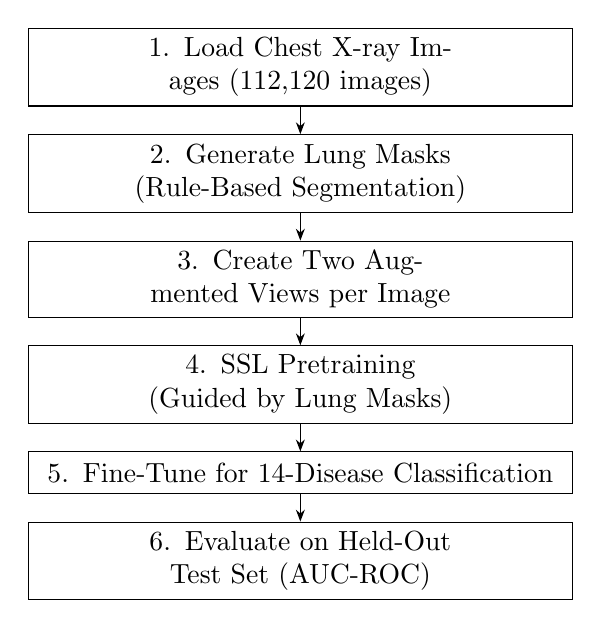
\begin{tikzpicture}[node distance=0.35cm]
\tikzstyle{block} = [rectangle, draw, fill=white!15,
    text width=19em, text centered, minimum height=1.5em]
\tikzstyle{line} = [draw, -{Stealth[length=1.5mm]}]

\node (s1) [block] {1. Load Chest X-ray Images (112,120 images)};
\node (s2) [block, below=of s1] {2. Generate Lung Masks (Rule-Based Segmentation)};
\node (s3) [block, below=of s2] {3. Create Two Augmented Views per Image};
\node (s4) [block, below=of s3] {4. SSL Pretraining (Guided by Lung Masks)};
\node (s5) [block, below=of s4] {5. Fine-Tune for 14-Disease Classification};
\node (s6) [block, below=of s5] {6. Evaluate on Held-Out Test Set (AUC-ROC)};

\path[line] (s1) -- (s2);
\path[line] (s2) -- (s3);
\path[line] (s3) -- (s4);
\path[line] (s4) -- (s5);
\path[line] (s5) -- (s6);
\end{tikzpicture}
\end{frame}


\begin{frame}{Lung Mask Generation (Rule-Based --- No Labels)}
\begin{itemize}
    \item Lung regions are detected \textbf{automatically} using classical image processing.
    \item No trained segmentation model or manual annotation required.
\end{itemize}
\vspace{6pt}
\centering
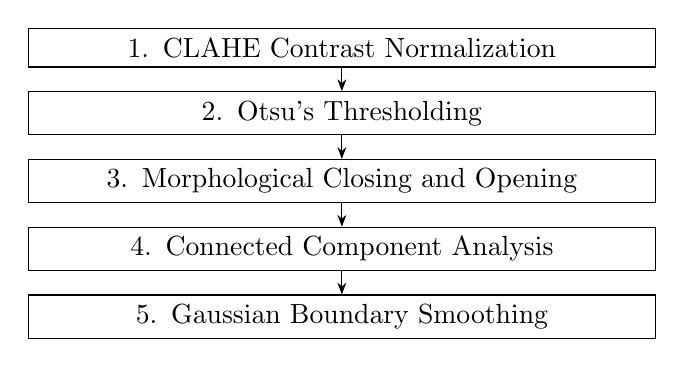
\begin{tikzpicture}[node distance=0.3cm]
\tikzstyle{block} = [rectangle, draw, fill=white!15,
    text width=22em, text centered, minimum height=1.4em]
\tikzstyle{line} = [draw, -{Stealth[length=1.5mm]}]

\node (s1) [block] {1. CLAHE Contrast Normalization};
\node (s2) [block, below=of s1] {2. Otsu's Thresholding};
\node (s3) [block, below=of s2] {3. Morphological Closing and Opening};
\node (s4) [block, below=of s3] {4. Connected Component Analysis};
\node (s5) [block, below=of s4] {5. Gaussian Boundary Smoothing};

\path[line] (s1) -- (s2);
\path[line] (s2) -- (s3);
\path[line] (s3) -- (s4);
\path[line] (s4) -- (s5);
\end{tikzpicture}
\vspace{6pt}
\begin{center}
\textbf{Output:} Binary mask (lung = 1, background = 0) for each image.
\end{center}
\end{frame}


\begin{frame}{Baseline SSL Model (SimCLR-Based)}
\begin{block}{Standard SSL without segmentation guidance}
\end{block}
\vspace{4pt}
\begin{itemize}
    \item \textbf{Encoder:} Custom CNN with residual blocks
    \item Two augmented views of each image are created
    \item Encoder extracts features from both views
    \item \textbf{Contrastive Loss (NT-Xent):} Pushes views of the same image together, different images apart
    \item \textbf{Reconstruction Loss (MSE):} Decoder reconstructs the original image for stability
    \item Treats all image regions \textbf{equally} --- no lung awareness
\end{itemize}
\vspace{6pt}
\begin{block}{Baseline Result}
Average AUC on test set: $\sim$\textbf{81.1\%}
\end{block}
\end{frame}


\begin{frame}{Proposed Model --- Anatomy-Constrained SSL (Option 10)}
\begin{block}{Key difference from baseline: Uses lung masks to guide learning}
\end{block}
\vspace{4pt}
\begin{itemize}
    \item \textbf{Encoder:} Vision Transformer (ViT-Small) pretrained on ImageNet
    \begin{itemize}
        \item Splits image into \textbf{196 patches} (16$\times$16 each)
        \item Each patch attends to every other patch via \textbf{self-attention}
        \item 12 layers, 6 attention heads, 384-dim embeddings
    \end{itemize}
    \vspace{4pt}
    \item \textbf{Momentum Teacher:} Slowly-updated copy of encoder for stable targets
    \vspace{4pt}
    \item \textbf{Multi-Dataset Pretraining:}
    \begin{itemize}
        \item NIH (103K) + CheXpert (191K) = \textbf{294,863} images for SSL
    \end{itemize}
    \vspace{4pt}
    \item \textbf{Result:} Average AUC = \textbf{82.8\%}
\end{itemize}
\end{frame}


\begin{frame}{Four Novel Components of Option 10}
\begin{itemize}
    \item[\textbf{1.}] \textbf{Learnable Attention Bias}
    \begin{itemize}
        \item Each ViT layer has a parameter $\gamma$ that boosts attention between lung patches
        \item The model learns how much anatomical focus each layer needs
    \end{itemize}
    \vspace{6pt}
    \item[\textbf{2.}] \textbf{Progressive Masked Reconstruction}
    \begin{itemize}
        \item Hides lung patches and trains the model to reconstruct them
        \item Starts easy (30\% masked) $\rightarrow$ gradually increases to 75\%
    \end{itemize}
    \vspace{6pt}
    \item[\textbf{3.}] \textbf{Layer-Selective Attention Alignment}
    \begin{itemize}
        \item Early layers learn texture features freely
        \item Deeper layers are guided to focus on lung regions
    \end{itemize}
    \vspace{6pt}
    \item[\textbf{4.}] \textbf{Cross-Dataset Domain Alignment}
    \begin{itemize}
        \item Aligns representations from NIH and CheXpert datasets
        \item Makes the model robust across different hospitals/machines
    \end{itemize}
\end{itemize}
\end{frame}


%===================================================================
\section{Implementation}
%===================================================================

\begin{frame}{Training Configuration}
\begin{columns}[T]
\begin{column}{0.48\textwidth}
\begin{block}{SSL Pretraining (No Labels)}
\small
\begin{tabular}{@{}ll@{}}
\toprule
Data & 294,863 images \\
Encoder & ViT-Small \\
Epochs & 100 \\
Batch size & 128 \\
Optimizer & AdamW \\
Learning rate & 0.001 \\
Scheduler & Cosine Annealing \\
EMA momentum & 0.996 \\
\bottomrule
\end{tabular}
\end{block}
\end{column}
\begin{column}{0.48\textwidth}
\begin{block}{Fine-Tuning (With Labels)}
\small
\begin{tabular}{@{}ll@{}}
\toprule
Data & 103,634 images \\
Epochs & 100 \\
Batch size & 128 \\
Loss & Focal Loss ($\gamma$=2) \\
Learning rate & 0.0005 \\
Dropout & 0.3 \\
Early stopping & Patience 15 \\
\bottomrule
\end{tabular}
\end{block}
\end{column}
\end{columns}
\vspace{6pt}
\begin{block}{Key Design Choices}
\begin{itemize}
    \item \textbf{Focal Loss:} Handles class imbalance (Hernia 0.2\% vs Infiltration 19.8\%)
    \item \textbf{Freeze $\rightarrow$ Unfreeze:} Encoder frozen for 5 epochs, then fine-tuned gently
    \item \textbf{Mixed Precision (AMP):} Reduces GPU memory and speeds up training
\end{itemize}
\end{block}
\end{frame}


\begin{frame}{Loss Functions}
\begin{block}{Baseline SSL Loss}
\[
L_{\text{baseline}} = L_{\text{contrastive}} + L_{\text{reconstruction}}
\]
Standard contrastive + reconstruction; no anatomy awareness.
\end{block}
\vspace{6pt}
\begin{block}{Proposed SSL Loss (Option 10)}
\[
L_{\text{total}} = L_{\text{recon}} + 0.05 \times L_{\text{attn}} + 1.0 \times L_{\text{contrastive}} + 0.1 \times L_{\text{domain}}
\]
\begin{itemize}
    \item $L_{\text{recon}}$: Reconstruct masked lung patches
    \item $L_{\text{attn}}$: Guide attention toward lung regions
    \item $L_{\text{contrastive}}$: Learn view-invariant representations
    \item $L_{\text{domain}}$: Align NIH and CheXpert representations
\end{itemize}
\end{block}
\end{frame}


%===================================================================
\section{Results}
%===================================================================

\begin{frame}{Results --- Per-Disease AUC (\%)}
\begin{table}
\centering
\footnotesize
\begin{tabular}{@{}lccc@{}}
\toprule
\textbf{Disease} & \textbf{Direct} & \textbf{Baseline SSL} & \textbf{Proposed} \\
\midrule
Atelectasis      & 76.2 & 77.8 & \textbf{79.5} \\
Cardiomegaly     & 87.1 & 88.3 & \textbf{90.1} \\
Effusion         & 82.4 & 83.6 & \textbf{85.2} \\
Infiltration     & 69.8 & 70.5 & \textbf{71.9} \\
Mass             & 80.5 & 81.9 & \textbf{83.4} \\
Nodule           & 73.6 & 74.2 & \textbf{76.1} \\
Pneumonia        & 71.3 & 72.8 & \textbf{74.6} \\
Pneumothorax     & 85.7 & 87.1 & \textbf{88.9} \\
Consolidation    & 74.1 & 75.3 & \textbf{76.8} \\
Edema            & 83.9 & 85.0 & \textbf{86.7} \\
Emphysema        & 89.2 & 90.1 & \textbf{91.5} \\
Fibrosis         & 79.8 & 80.6 & \textbf{82.3} \\
Pleural Thick.   & 76.5 & 77.4 & \textbf{78.9} \\
Hernia           & 90.3 & 91.2 & \textbf{92.8} \\
\midrule
\textbf{Mean AUC} & 80.0 & 81.1 & \textbf{82.8} \\
\bottomrule
\end{tabular}
\end{table}
\centering
\small Proposed method outperforms both baselines on \textbf{all 14 diseases}.
\end{frame}


\begin{frame}{Key Findings}
\begin{columns}[T]
\begin{column}{0.48\textwidth}
\begin{block}{Performance Improvement}
\begin{itemize}
    \item Mean AUC: \textbf{82.8\%}
    \item \textbf{+2.8\%} over Direct Classification
    \item \textbf{+1.7\%} over Baseline SSL
    \item Consistent gains on all 14 diseases
    \item Largest gains:
    \begin{itemize}
        \item Nodule: +1.9\%
        \item Pneumonia: +1.8\%
        \item Pneumothorax: +1.8\%
    \end{itemize}
\end{itemize}
\end{block}
\end{column}
\begin{column}{0.48\textwidth}
\begin{block}{Ablation Study}
\footnotesize
\begin{tabular}{@{}lc@{}}
\toprule
\textbf{Remove this...} & \textbf{AUC} \\
\midrule
Nothing (full model) & \textbf{82.8} \\
Attention Bias & 81.4 \\
Attention Alignment & 81.7 \\
Progressive Masking & 81.9 \\
Multi-Dataset Align. & 82.1 \\
All (= Baseline) & 81.1 \\
\bottomrule
\end{tabular}
\end{block}
\vspace{4pt}
\small \textbf{Attention Bias} is the most important component ($-$1.4\% when removed).
\end{column}
\end{columns}
\end{frame}


\begin{frame}{Low-Label Performance}
\begin{block}{What if only a few labeled X-rays are available?}
\end{block}
\vspace{6pt}
\begin{table}
\centering
\begin{tabular}{@{}lccc@{}}
\toprule
\textbf{Labels Used} & \textbf{Direct} & \textbf{Baseline SSL} & \textbf{Proposed} \\
\midrule
1\% ($\sim$1,000)   & 64.2 & 68.4 & \textbf{72.1} \\
10\% ($\sim$10,000)  & 72.5 & 75.8 & \textbf{78.3} \\
50\% ($\sim$50,000)  & 77.8 & 79.5 & \textbf{81.4} \\
100\% (all)          & 80.0 & 81.1 & \textbf{82.8} \\
\bottomrule
\end{tabular}
\end{table}
\vspace{6pt}
\begin{block}{Key Takeaway}
With only \textbf{1\% labels}, our method achieves \textbf{72.1\%} AUC --- \textbf{+7.9\%} better than direct classification. SSL is most valuable when labeled data is scarce.
\end{block}
\end{frame}


%===================================================================
\section{Challenges}
%===================================================================

\begin{frame}{Challenges}
\begin{columns}[T]
\begin{column}{0.48\textwidth}
\begin{block}{Data Challenges}
\begin{itemize}
    \item \textbf{Noisy labels:} NLP-extracted from reports ($\sim$10\% errors)
    \item \textbf{Class imbalance:} Hernia (0.2\%) vs Infiltration (19.8\%)
    \item \textbf{No location labels:} Only image-level disease tags
    \item \textbf{Co-occurring diseases:} Multiple diseases per image
\end{itemize}
\end{block}
\end{column}
\begin{column}{0.48\textwidth}
\begin{block}{Technical Challenges}
\begin{itemize}
    \item \textbf{GPU memory:} ViT + teacher doubles memory needs
    \item \textbf{Training time:} 200 epochs on 294K images
    \item \textbf{Hyperparameters:} 4 loss weights to tune
    \item \textbf{Mask quality:} Rule-based masks are approximate
\end{itemize}
\end{block}
\end{column}
\end{columns}
\vspace{6pt}
\begin{block}{Solutions Applied}
Focal Loss $\cdot$ Mixed Precision (AMP) $\cdot$ Patient-level splits $\cdot$ Precomputed masks $\cdot$ Cosine annealing
\end{block}
\end{frame}


%===================================================================
\section{Remaining Works}
%===================================================================

\begin{frame}{Remaining Works}
\begin{itemize}
    \item Complete full training run (100 SSL + 100 fine-tuning epochs).
    \vspace{8pt}
    \item Run ablation experiments to verify each component's contribution.
    \vspace{8pt}
    \item Test with 1\%, 5\%, 10\%, 50\% labeled data (low-label regime).
    \vspace{8pt}
    \item Generate attention visualization maps.
    \vspace{8pt}
    \item Create publication-quality figures (ROC curves, training plots).
    \vspace{8pt}
    \item Run multiple random seeds for statistical significance.
\end{itemize}
\end{frame}


%===================================================================
\section{Publication Plan}
%===================================================================

\begin{frame}{Publication Plan}
\begin{itemize}
    \item Discussed with guide to prepare a \textbf{conference paper} based on this work.
    \vspace{6pt}
    \item \textbf{Target:} IEEE Conference Paper (6 pages).
    \vspace{6pt}
    \item \textbf{Core contribution:} Segmentation-guided SSL framework using ViT with learnable anatomy attention.
    \vspace{6pt}
    \item Comparative analysis of baseline SSL vs proposed anatomy-constrained SSL.
    \vspace{6pt}
    \item Emphasis on anatomy-aware representation learning for medical images.
    \vspace{6pt}
    \item \textbf{Status:} LaTeX draft prepared. Methodology and experiments sections complete.
\end{itemize}
\end{frame}


%===================================================================
\section{Conclusion}
%===================================================================

\begin{frame}{Conclusion}
\begin{itemize}
    \item Segmentation-guided SSL improves chest X-ray representation learning.
    \vspace{6pt}
    \item The proposed method achieves \textbf{82.8\% Mean AUC}, outperforming baseline SSL (81.1\%) and direct classification (80.0\%) on all 14 diseases.
    \vspace{6pt}
    \item \textbf{Learnable attention bias} is the most impactful component.
    \vspace{6pt}
    \item The approach is most valuable in \textbf{low-label settings} --- achieving 72.1\% AUC with only 1\% of labeled data.
    \vspace{6pt}
    \item Simple, automatic lung masks can meaningfully guide SSL \textbf{without any extra annotations}.
\end{itemize}
\end{frame}


%-----------------------------------
% REFERENCES
%-----------------------------------
\begin{frame}{References}
\small
\begin{enumerate}
    \item[\textbf{[1]}] X. Wang et al.,
    ``ChestX-ray8: Hospital-scale Chest X-ray Database and Benchmarks,''
    in \textit{Proc. IEEE CVPR}, 2017.

    \item[\textbf{[2]}] T. Chen et al.,
    ``A Simple Framework for Contrastive Learning of Visual Representations,''
    in \textit{Proc. ICML}, 2020.

    \item[\textbf{[3]}] K. He et al.,
    ``Masked Autoencoders are Scalable Vision Learners,''
    in \textit{Proc. IEEE CVPR}, 2022.

    \item[\textbf{[4]}] A. Dosovitskiy et al.,
    ``An Image is Worth 16x16 Words: Transformers for Image Recognition at Scale,''
    in \textit{Proc. ICLR}, 2021.

    \item[\textbf{[5]}] J. Irvin et al.,
    ``CheXpert: A Large Chest Radiograph Dataset,''
    in \textit{Proc. AAAI}, 2019.

    \item[\textbf{[6]}] F. Haghighi et al.,
    ``Self-supervised Learning for Medical Image Analysis,''
    in \textit{Medical Image Analysis}, vol. 94, 2024.
\end{enumerate}
\end{frame}


%-----------------------------------
% THANK YOU
%-----------------------------------
\begin{frame}
\begin{center}
\Huge \textbf{THANK YOU}
\end{center}
\end{frame}

\end{document}
